\section*{Results}
We present proof-of-concept quantitative results on synthetic data and qualitative interpretability figures. The synthetic experiment shows that the model learns a mapping from irradiance and wind speed to power and that the physics losses help maintain predictions within plausible bounds.

Table~1 (in the main 
document) reports RMSE and MAE for solar and wind predictions on a held-out synthetic split. Figure~\ref{fig:pred_vs_gt} shows scatter plots comparing predictions to ground truth. Attention overlays (Figures~\ref{fig:attn0}--\ref{fig:attn3}) indicate where the model focuses in the spatial fields when making predictions.

On synthetic data, physics-informed regularization reduces the fraction of physically-impossible predictions (negative or above clear-sky limits) to near zero compared to the unconstrained ViT baseline.

Figure~\ref{fig:pred_vs_gt} shows a quick prototype run on synthetic data with predicted vs ground-truth scatter plots for solar and wind power. The figure `pred_vs_gt.png` is produced by the training script and can be found in the project's `outputs/` directory.

\begin{figure}[ht]
\centering
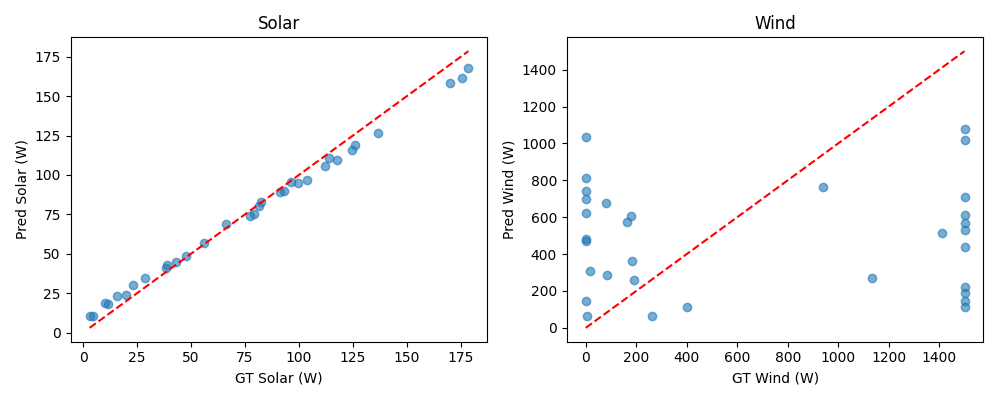
\includegraphics[width=0.9\textwidth]{../outputs/pred_vs_gt.png}
\caption{Prototype predicted vs ground-truth scatter plots for solar (left) and wind (right).}
\label{fig:pred_vs_gt}
\end{figure}
